\documentclass[aspectratio=169,12pt]{beamer}
\usepackage[utf8]{inputenc}
\usepackage{amsmath, amssymb}
\usepackage{booktabs}
\usepackage{colortbl}
\usepackage{hyperref}
\usepackage{makecell}
\usepackage{ragged2e}
\usepackage{bytefield}
\usepackage{tikz}
\usepackage{circuitikz}
\usetikzlibrary{arrows.meta, positioning, shapes.geometric, calc, tikzmark, shapes.misc, automata, matrix}
\usepackage{tcolorbox}
\usepackage{listings}
\usepackage{pifont}
\usetheme{Madrid}

\lstset{
    basicstyle=\ttfamily\small,
    keywordstyle=\color{blue}\bfseries,
    commentstyle=\color{gray},
    stringstyle=\color{red},
    numbers=left,
    numberstyle=\tiny\color{gray},
    stepnumber=1,
    numbersep=5pt,
    backgroundcolor=\color{white},
    showspaces=false,
    showstringspaces=false,
    showtabs=false,
    frame=single,
    tabsize=2,
    captionpos=b,
    breaklines=true,
    breakatwhitespace=false,
    escapeinside={(*@}{@*)},
}

\newcommand{\xmark}{\ding{55}} % Cross mark

% Define colors for pipeline diagrams
\definecolor{normalexec}{RGB}{46, 125, 50}
\definecolor{stallcolor}{RGB}{255, 193, 7}
\definecolor{flushcolor}{RGB}{211, 47, 47}
\definecolor{emptycolor}{RGB}{238, 238, 238}

% Program code - can't be in macro due to lstlisting limitations

% 4-state machine macro
\newcommand{\fourstatemachine}[1][0.6]{
\begin{tikzpicture}[scale=#1, node distance=2.5cm, auto]
    \node[state, fill=red!20] (00) {00};
    \node[state, fill=orange!20, draw=blue, thick, right of=00] (01) {01};
    \node[state, fill=yellow!20, right of=01] (10) {10};
    \node[state, fill=green!20, right of=10] (11) {11};
    
    \path[->] 
    (00) edge[loop left] node{\tiny NT} (00)
    (00) edge[above, bend left] node{\tiny T} (01)
    (01) edge[below, bend left] node{\tiny NT} (00)
    (01) edge[above, bend left] node{\tiny T} (10)
    (10) edge[below, bend left] node{\tiny NT} (01)
    (10) edge[above, bend left] node{\tiny T} (11)
    (11) edge[below, bend left] node{\tiny NT} (10)
    (11) edge[loop right] node{\tiny T} (11);
\end{tikzpicture}
}

% Prediction table macro with progressive revelation
\newcommand{\predictiontable}{
\begin{table}
\centering
\scriptsize
\begin{tabular}{|c|c|c|c|c|c|c|c|}
\hline
\textbf{Cycle} & \textbf{R1} & \textbf{R2} & \textbf{Current} & \textbf{Prediction} & \textbf{Actual} & \textbf{Next} & \textbf{Misprediction} \\
 & & & \textbf{State} & & & \textbf{State} & \\
\hline
Loop1 & 2 & 2 & & & & & \\
\hline
\pause BNEQ & 2 & 1 & 01 & not taken & taken & 10 & \checkmark \\
\hline
\pause BNEQ & 2 & 0 & 10 & taken & not taken & 01 & \checkmark \\
\hline
\pause Loop1 & 3 & 3 & & & & & \\
\hline
\pause BNEQ & 3 & 2 & 01 & not taken & taken & 10 & \checkmark \\
\hline
\pause BNEQ & 3 & 1 & 10 & taken & taken & 11 & \\
\hline
\pause BNEQ & 3 & 0 & 11 & taken & not taken & 10 & \checkmark \\
\hline
\end{tabular}
\end{table}
}

% BTB Structure diagram macro
\newcommand{\btbdiagram}{
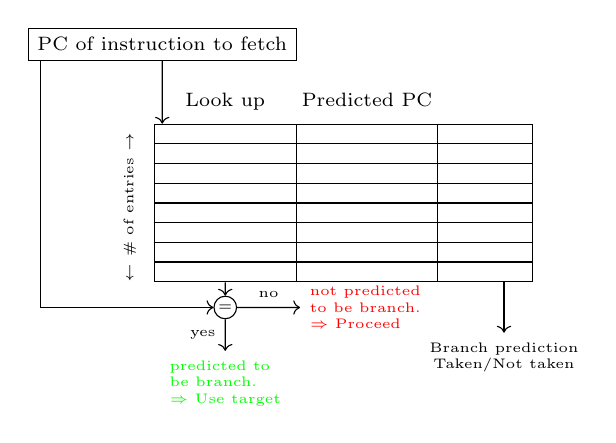
\begin{tikzpicture}[scale=0.8]
    % BTB table as matrix using your style
    \matrix[matrix of nodes,
            column sep=-\pgflinewidth,
            row sep=-\pgflinewidth,
            inner sep=0pt,
            anchor=north,
            nodes in empty cells,
            nodes={draw, align=center},
            column 1/.append style={nodes={text width=1.8cm, minimum height=0.25cm}},
            column 2/.append style={nodes={text width=1.8cm, minimum height=0.25cm}},
            column 3/.append style={nodes={text width=1.2cm, minimum height=0.25cm}},
            ampersand replacement=\&
        ] (btb) {
        \& \& \\
        \& \& \\
        \& \& \\
        \& \& \\
        \& \& \\
        \& \& \\
        \& \& \\
        \& \& \\
    };
    
    \node[draw, rectangle, above=8mm of btb-1-1.north, xshift=-8mm, font=\scriptsize] (pc) {PC of instruction to fetch};
    % Table headers positioned relative to matrix columns
    \node[above=1mm of btb-1-1.north, text depth=0ex, font=\scriptsize] {Look up};
    \node[above=1mm of btb-1-2.north, text depth=0ex, font=\scriptsize] {Predicted PC};
    
    % BTB label positioned relative to matrix left
    \node[rotate=90, left=5mm of btb.north west, font=\tiny, anchor=north east] {$\leftarrow$ \# of entries $\rightarrow$};
    
    % Comparator positioned relative to first column bottom
    \node[circle, draw, inner sep=1pt, font=\tiny] (comp) at ($ (btb-8-1.south) + (0, -0.4) $) {=};
    
    % Arrows using relative positioning
    \draw[->] (pc) -- (btb-1-1.north -| pc);
    \draw[->] ([xshift=2mm]pc.south west) |- (comp.west);
    \draw[->] (btb-8-1.south) -- (comp);

    \node[right=8mm of comp, font=\tiny, align=left, text=red] (no) {not predicted\\to be branch.\\ $\Rightarrow$ Proceed};

    % Output logic positioned relative to comparator
    \draw[->] (comp.east) -- node[above, font=\tiny]{no} (no);

    \node[below=4mm of comp, font=\tiny, align=left, text=green] (yes) {predicted to\\be branch.\\ $\Rightarrow$ Use target};
    \draw[->] (comp.south) -- node[left, font=\tiny]{yes} (yes);
    
    % Prediction output from third column
    \draw[->] ([xshift=3mm]btb-8-3.south) -- ++(0, -8mm) node[below, align=center, font=\tiny] {Branch prediction\\Taken/Not taken};
\end{tikzpicture}
}

\title{Data and Control Hazards}
\author{Compuetr Architecture 234267}
\date{2025, Recitation \#2}

\begin{document}

\frame{\titlepage}

\begin{frame}{Pipeline Processor with Hazard Detection}
\centering
\scalebox{0.7}{%
\begin{circuitikz}[
    % Component styles - avoid using scale
    component/.style={draw, thick, minimum height=0.8cm},
    pipeline_reg/.style={draw, thick, fill=gray!20, minimum width=6mm, minimum height=7.4cm},
    stage_label/.style={draw, thick, fill=blue!60, text=white, font=\bfseries, minimum width=0.8cm, minimum height=0.5cm},
    control_block/.style={draw, thick, fill=orange!30, rounded corners=3pt, font=\small},
    hazard_unit/.style={muxdemux, muxdemux def={Lh=1.5, NL=2, Rh=1.5, NR=3, NB=6, w=2.5, square pins=1}, 
                       external pins width=0, fill=red!60, text=white},
    memory_block/.style={muxdemux, muxdemux def={Lh=6, NL=1, Rh=6, NR=1, w=4, square pins=1}, 
                        external pins width=0, align=center, text depth=8ex},
    regfile/.style={muxdemux, muxdemux def={Lh=7, NL=5, Rh=7, NR=2, NB=1, w=3.2, square pins=1}, 
                    external pins width=0, fill=cyan!20, align=center},
    alu_style/.style={muxdemux, muxdemux def={Lh=5, NL=2, Rh=2, NR=1, w=1.2, inset w=0.5, inset Lh=2, inset Rh=0, square pins=1},
                     external pins width=0, fill=green!20},
    mux2/.style={muxdemux, muxdemux def={Lh=3, Rh=1.5, NL=2, NR=1, NB=1, w=1}, 
                 external pins width=0},
    mux3/.style={muxdemux, muxdemux def={Lh=4, Rh=2, NL=3, NR=1, NB=1, w=1}, 
                 external pins width=0},
    mux4/.style={muxdemux, muxdemux def={Lh=2, Rh=1, NL=2, NR=1, NB=1, w=1}, 
                 external pins width=0},
    arrow/.style={->, >=stealth, thick},
    data_path/.style={arrow, black},
    control_path/.style={arrow, orange!70},
    hazard_path_input/.style={arrow, red!70},
    hazard_path/.style={arrow, red!70, dashed},
    forward_path/.style={arrow, orange!50},
    control_signal/.style={draw, thick, fill=orange!30, minimum width=6mm, minimum height=0.3cm, font=\scriptsize},
    data_latch/.style={draw, thick, fill=cyan!20, minimum width=6mm, minimum height=0.3cm, font=\scriptsize},
    % Connector circles
    black_connector/.style={circle, fill, inner sep=1.2pt},
    red_connector/.style={circle, fill, inner sep=1.2pt, red!70},
    % Path labels
    path_label/.style={font=\tiny, midway, above, yshift=-2},
    control_label/.style={path_label, text=orange!70},
    node distance=5mm and 5mm,
]

%\ctikzset{font=\scriptsize}

% Define origin
\coordinate (origin) at (0,0);

% IF Stage Components
% Instruction Memory using muxdemux
%\node[memory_block, fill=yellow!20] (IMem) at (IFID.west) [anchor=east, xshift=-0.5cm] {Instruction\\Memory};
\node[component, fill=yellow!30, minimum width=0.8cm] (PC) {PC};
\node[memory_block, fill=yellow!20, right=of PC] (IMem) {Instruction\\Memory};
\node[pipeline_reg, right=of IMem] (IFID) {};


% Small labels on pipeline registers
%\node[font=\tiny, rotate=90] at (IFID.center) {IF/ID};
%\node[font=\tiny, rotate=90] at (IDEX.center) {ID/EX};
%\node[font=\tiny, rotate=90] at (EXMEM.center) {EX/MEM};
%\node[font=\tiny, rotate=90] at (MEMWB.center) {MEM/WB};


% ID Stage Components
% Register File using muxdemux style
\node[regfile, right=1.5cm of IFID] (RegFile) {Register\\File};
% Add labels to RegFile pins

% Control Unit
\node[control_block, ellipse, minimum height=0.5cm, minimum width=0.5cm,
      above=1mm of RegFile] (Control) {\rotatebox{90}{Control}};

% Hazard Detection Unit
\node[hazard_unit, above=of Control.north west, yshift=-2mm, xshift=-9mm] (HDU) {HDU};

% AND gate for HDU control
\node[and port, anchor=bin 2, fill=red!60, scale=0.5, external pins width=0] (HDU_AND) at ([xshift=5mm]Control.east) {};
\node[pipeline_reg, right=10mm of RegFile] (IDEX) {};

% EX Stage Components
\node[mux2, fill=orange!20, anchor=blpin 1] (ForwardA) at ([xshift=10mm]IDEX.east |- RegFile.brpin 1) {};
\node[alu_style, right=of ForwardA.brpin 1, anchor=blpin 1] (ALU) {\rotatebox{90}{ALU}};
\node[mux2, fill=orange!20, anchor=blpin 1] (ForwardB) at ([xshift=10mm]IDEX.east |- RegFile.brpin 2) {};

% Register fields in IDEX latch (bottom to top)
\node[data_latch] (Rd_field) at ([yshift=2mm]IDEX.south) {\tiny Rd};
\node[mux4, fill=cyan!20, anchor=blpin 2] (RegDstMux) at ([xshift=-3mm]ForwardB.blpin 2 |- Rd_field.east) {};
\node[data_latch, font=\tiny] (Rt_field) at (RegDstMux.lpin 1 -| Rd_field) {Rt};
\node[data_latch, anchor=south, font=\tiny] (Rs_field) at ([yshift=1mm]Rt_field.north) {Rs};

% Forwarding Unit
\node[muxdemux, muxdemux def={Lh=1.6, NL=4, Rh=1.6, NR=4, w=3, square pins=1}, 
      external pins width=0, fill=orange!30, font=\scriptsize, align=center, below right=5mm of RegDstMux.east] (FwdUnit) {Forwarding\\Unit};

\node[pipeline_reg] (EXMEM) at ([xshift=1cm]ALU.east |- IDEX) {};

% MEM Stage Components


% Data Memory using muxdemux
\node[memory_block, fill=yellow!20, anchor=blpin 1, align=center] (DMem) at ([xshift=5mm]EXMEM.east |- ALU) {Data\\Memory};
\node[pipeline_reg] (MEMWB) at ([xshift=5mm]DMem.east |- EXMEM) {};

% WB Stage Components
\node[mux2, fill=cyan!20, right=of MEMWB, anchor=blpin 1] (WBMux) {};


% Control signal blocks in pipeline registers
\node[control_signal] (WB1) at ([yshift=-2mm]IDEX.north) {\tiny WB};
\node[control_signal] (M1) at (WB1.south) [anchor=north, yshift=-0.1cm] {\tiny M};
\node[control_signal] (EX1) at (M1.south) [anchor=north, yshift=-0.1cm] {\tiny EX};

\node[control_signal] (WB2) at (WB1 -| EXMEM.center) {\tiny WB};
\node[control_signal] (M2) at (WB2.south) [anchor=north, yshift=-0.1cm] {\tiny M};

\node[control_signal] (WB3) at (WB1 -| MEMWB.center) {\tiny WB};


% Register fields in EXMEM and MEMWB latches
\node[data_latch] (EXMEM_RtRd) at (EXMEM |- RegDstMux.rpin 1) {\rotatebox{90}{\tiny Rt/Rd}};
\node[data_latch] (MEMWB_RtRd) at (MEMWB |- EXMEM_RtRd) {\rotatebox{90}{\tiny Rt/Rd}};

% Main data paths
% PC to Instruction Memory
\draw[data_path] (PC.east) -- (IMem.west);
% Instruction Memory to IF/ID
\draw[data_path] (IMem.east) -- (IFID.west);

% IF/ID to Register File
\draw[data_path] (IFID.east) -- ++(0.3,0) |- node[path_label, pos=0.9] {Rs} (RegFile.blpin 1);
\draw[data_path] (IFID.east) -- ++(0.3,0) |- node[path_label, pos=0.9] {Rt} (RegFile.blpin 2);
\draw[data_path] (IFID.east) -- ++(0.3,0) |- node[path_label, pos=0.8] {Rd} (Rd_field.west);
\draw[data_path] ([xshift=-9mm]RegFile.blpin 1) node[black_connector] {}
                    |- node[path_label, pos=0.8] {Rs} (Rs_field.west);  
\draw[data_path] ([xshift=-10mm]RegFile.blpin 2) node[black_connector] {}
                    |- node[path_label, pos=0.8] {Rt} (Rt_field.west);  


\draw[data_path] (IFID.east) -- ++(0.3,0) |- (Control.west);

% Register File outputs to ID/EX
\draw[data_path] (RegFile.brpin 1) -- (RegFile.brpin 1 -| IDEX.west);
\draw[data_path] (RegFile.brpin 2) -- (RegFile.brpin 2 -| IDEX.west);

% ID/EX to EX stage (through forwarding muxes)
\draw[data_path] (IDEX.east |- RegFile.brpin 1) -- (ForwardA.blpin 1);
\draw[data_path] (IDEX.east |- RegFile.brpin 2) -- (ForwardB.blpin 1);

% Forwarding muxes to ALU
\draw[data_path] (ForwardA.brpin 1) -- (ALU.blpin 1);
\draw[data_path] (ForwardB.brpin 1) -- (ALU.blpin 2);

% TODO: add comment
\draw[data_path] (Rt_field.east) -- (RegDstMux.blpin 1);
\draw[data_path] (Rd_field.east) -- (RegDstMux.blpin 2);
\draw[data_path] (RegDstMux.brpin 1) --  (EXMEM_RtRd.west);
\draw[data_path] (EXMEM_RtRd.east) -- node[near end, above, font=\tiny] {RegDst} (MEMWB_RtRd.west);
\draw[data_path]
  (MEMWB_RtRd.east) -- ++(0.5,0)
  |- ([yshift=-9mm]FwdUnit.south)
  -| node[path_label, above right]{RegDst} ([xshift=-8mm]RegFile.blpin 3)
  -- node[path_label]{RegDst} % or pos=0.9, etc.
     (RegFile.blpin 3);

% ALU to EX/MEM
\draw[data_path] (ALU.east) -- (EXMEM.west |- ALU.east);

% EX/MEM to Data Memory
\draw[data_path] (EXMEM.east |- ALU) -- (DMem.blpin 1);
\draw[data_path] ([xshift=3mm]EXMEM.east |- ALU)  node[black_connector] {} 
    |- ([yshift=-5mm]DMem.south)
    -- ([yshift=-5mm]MEMWB.west |- DMem.south);

% Data Memory to MEM/WB
\draw[data_path] (DMem.east) -- (MEMWB.west |- DMem.east);

% MEM/WB to WB Mux
\draw[data_path] (MEMWB.east) -- (WBMux.blpin 1);
\draw[data_path] ([yshift=-5mm]MEMWB.east |- DMem.south) -- ++(0.3,0) |- (WBMux.blpin 2);

% Write back path
\draw[data_path]
  (WBMux.brpin 1) -- ++(0.5,0)
  |- ([yshift=-5mm]FwdUnit.south)
  -| node[path_label, above right]{WrData} ([xshift=-7mm]RegFile.blpin 4)
  -- node[path_label]{WrData} % or pos=0.9, etc.
     (RegFile.blpin 4);

% Control paths
\draw[control_path] (HDU_AND.bout) -- ++(0.3, 0) |- (M1.west);
\draw[control_path] (HDU_AND.bout) -- ++(0.3, 0) |- (WB1.west);
\draw[control_path] (HDU_AND.bout) -- ++(0.3, 0) |- (EX1.west);
\draw[control_path] (Control.east) -- (HDU_AND.bin 2);
\draw[control_path] (WB1.east) -- (WB2.west);
\draw[control_path] (M1.east) -- (M2.west);
\draw[control_path] (WB2.east) -- (WB3.west);
\draw[control_path]
    (WB3.east) -- ++(0.2, 0)
    |- node[pos=0.1, right, font=\tiny] {RegWrite} ([yshift=-2mm]FwdUnit.south)
    -| node[control_label, above right] {RegWrite} ([xshift=-4mm]RegFile.blpin 5)
    -- (RegFile.blpin 5);

% Hazard detection paths
%\draw[hazard_path] ([xshift=-0.2cm]RegFile.south) |- ([yshift=-0.3cm]HDU.blpin 2);
%\draw[hazard_path] ([xshift=0.2cm]RegFile.south) |- ([yshift=0.3cm]HDU.west);
\draw[hazard_path] (HDU.brpin 3) -- ++(1, 0) |- (HDU_AND.bin 1);
\draw[hazard_path] (HDU.blpin 1) -| (PC.north);
\draw[hazard_path] (HDU.blpin 2) -| (IFID.north);
\draw[hazard_path_input] (RegFile.blpin 2 -| HDU.bbpin 2) node[red_connector] {} -- (HDU.bbpin 2);
\draw[hazard_path_input] (RegFile.blpin 1 -| HDU.bbpin 3) node[red_connector] {} -- (HDU.bbpin 3);
\draw[hazard_path_input] ([xshift=-1cm]M2.west) node[red_connector] {} |- (HDU.brpin 2);
\draw[hazard_path_input] ([xshift=-3mm]EXMEM_RtRd.west) node[red_connector] {} |- (HDU.brpin 1);

% Forwarding paths
%\draw[forward_path] (EXMEM.south) |- ([yshift=-0.3cm]FwdUnit.west);
%\draw[forward_path] (MEMWB.south) |- ([yshift=0.3cm]FwdUnit.west);
%\draw[forward_path] ([yshift=0.3cm]FwdUnit.east) |- (ForwardA.south);
%\draw[forward_path] ([yshift=-0.3cm]FwdUnit.east) |- (ForwardB.south);
\draw[forward_path] (FwdUnit.blpin 1) -- ++(-0.1, 0)
    -| ([xshift=1mm, yshift=-3mm]ForwardB.east)
    |- ([yshift=-3mm]ForwardA.bbpin 1)
    -- (ForwardA.bbpin 1);

\draw[forward_path] (FwdUnit.blpin 2) -- ++(-0.2, 0)
    |- ([yshift=-3mm]ForwardB.bbpin 1)
    -- (ForwardB.bbpin 1);

\draw[data_path] (Rs_field.east) -- ++(0.3,0) |- (FwdUnit.blpin 3);
\draw[data_path] ([xshift=2mm]Rt_field.east) node[black_connector] {}  |- (FwdUnit.blpin 4);

% Add some labels

% Stage labels at top (after pipeline registers are defined)
%\node[stage_label] (IF_label) at (0, 4) {IF};
%\node[stage_label] (ID_label) at ($ (IFID.center)!0.5!(IDEX.center) $ |- IF_label) {ID};
%\node[stage_label] (EX_label) at ($ (IDEX.center)!0.5!(EXMEM.center) $ |- IF_label) {EX};
%\node[stage_label] (MEM_label) at ($ (EXMEM.center)!0.5!(MEMWB.center) $ |- IF_label) {MEM};
%\node[stage_label] (WB_label) at (13, 4) {WB};


% Instructions in pipeline (as text annotations)
%\node[font=\scriptsize, text=green!60!black, anchor=west] at (13.5, 1) {ADD \$6 ← \$6 \$7};
%\node[font=\scriptsize, text=red!60!black, anchor=west] at (13.5, 0.5) {SUB \$4 ← \$5 \$1};
%\node[font=\scriptsize, text=blue!60!black, anchor=west] at (13.5, 0) {LW \$1 ← 100(\$4)};

% Instruction addresses
%\node[font=\tiny, text=blue!60!black] at (14, -1) {100: LW \$1←(100)(\$4)};
%\node[font=\tiny, text=blue!60!black] at (14, -1.3) {104: SUB \$4 ← \$5 \$1};
%\node[font=\tiny, text=blue!60!black] at (14, -1.6) {108: Add \$6 ← \$6 \$7};

\end{circuitikz}
}
\end{frame}



\begin{frame}{Control Hazards Solutions - Branch Target Buffer (BTB)}
\textbf{Direction Prediction (Taken/Not Taken):}
\begin{columns}
\column{0.5\textwidth}
\begin{itemize}
    \item Remembers branch behavior from recent executions
    \item If taken recently, predict taken again
    \item Uses state machines for history
\end{itemize}

\column{0.5\textwidth}
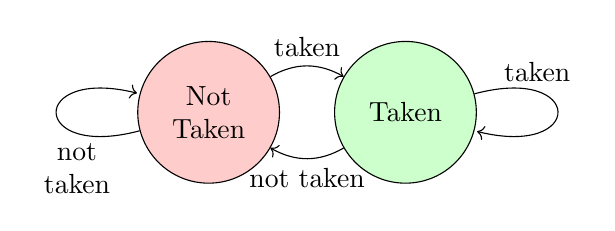
\begin{tikzpicture}[scale=0.8, node distance=2.5cm]
    \node[state, fill=red!20, minimum size=1.8cm, align=center] (nt) {Not\\Taken};
    \node[state, fill=green!20, minimum size=1.8cm, align=center, right of=nt] (t) {Taken};
    
    \path[->] 
    (nt) edge[bend left, above] node{taken} (t)
    (t) edge[bend left, below] node{not taken} (nt)
    (nt) edge[loop left] node[below, align=center, near start] {not\\taken} (nt)
    (t) edge[loop right] node[above, align=center, near start]{taken} (t);
\end{tikzpicture}
\end{columns}
\vspace{0.5cm}
\textbf{Target Address Prediction:}
\begin{itemize}
    \item Also remembers the jump target address
\end{itemize}

\begin{tcolorbox}[colback=yellow!10]
\small
Note: Initial state is "not taken" because on first encounter with a branch instruction, the target address is unknown. Only after the branch jumps for the first time can we store its target address.
\end{tcolorbox}
\end{frame}

\begin{frame}{Enhanced Prediction with 2-bit State Machine}
\textbf{More reliable prediction using 4-state machine:}

\begin{center}
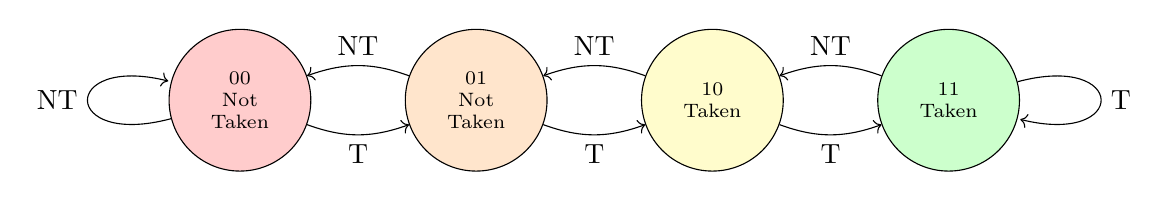
\begin{tikzpicture}[scale=1, node distance=3cm, auto]
    % Define states with minimum size
    \node[state, fill=red!20, align=center, minimum size=1.8cm, font=\scriptsize] (00) {00\\Not\\Taken};
    \node[state, fill=orange!20, right of=00, align=center, minimum size=1.8cm, font=\scriptsize] (01) {01\\Not\\Taken};
    \node[state, fill=yellow!20, right of=01, align=center, minimum size=1.8cm, font=\scriptsize] (10) {10\\Taken};
    \node[state, fill=green!20, right of=10, align=center, minimum size=1.8cm, font=\scriptsize] (11) {11\\Taken};
    
    % Add transitions with loops on left and right
    \path[->] 
    % From 00
    (00) edge[loop left] node{NT} (00)
    (00) edge[below, bend right=20] node{T} (01)
    % From 01
    (01) edge[above, bend right=20] node{NT} (00)
    (01) edge[below, bend right=20] node{T} (10)
    % From 10
    (10) edge[above, bend right=20] node{NT} (01)
    (10) edge[below, bend right=20] node{T} (11)
    % From 11
    (11) edge[above, bend right=20] node{NT} (10)
    (11) edge[loop right] node{T} (11);
    
    % Add direction arrows
   % \draw[thick, ->, blue] (0, -1.5) -- (12, -1.5) node[right, align=center] {Taken};
   % \draw[thick, ->, red] (0, -2) -- (12, -2) node[right, align=center] {Not\\Taken};
\end{tikzpicture}
\end{center}

\textbf{Key advantages:}
\begin{itemize}
    \item States 00 and 11 are stable states
    \item Transition to opposite prediction only after TWO consecutive mispredictions
    \item Reduces impact of irregular jumps/exceptions
    \item Initial state set to 01 (not taken, unstable)
\end{itemize}
\end{frame}

\begin{frame}{Branch Target Buffer (BTB) Structure - Overview}
\begin{columns}
\column{0.5\textwidth}
\centering
\btbdiagram

\column{0.5\textwidth}

\vspace{0.3cm}
\textbf{Lookup Process:}
\begin{enumerate}
    \item Compare PC with stored addresses/tags
    \item If match found: use prediction and target
    \item If no match: assume not a branch
\end{enumerate}

\vspace{0.3cm}
\textbf{Limitation:}
\begin{itemize}
    \item May store partial addresses (tags) to save space
    \item Can cause \textcolor{red}{false matches} $\Rightarrow$ mispredictions
\end{itemize}
\end{columns}
\end{frame}

\begin{frame}{BTB Structure - Components}
\begin{columns}
\column{0.5\textwidth}
\centering
\btbdiagram

\column{0.5\textwidth}
\textbf{BTB Fields:}
\begin{itemize}
    \item \textbf{Left field:} Branch address/tag
    \begin{itemize}
        \item May use hash or partial address
        \item \textcolor{red}{Tag conflicts} can cause errors
    \end{itemize}
    \item \textbf{Middle field:} Target address
    \begin{itemize}
        \item Populated after first branch execution
        \item Used when prediction is "taken"
    \end{itemize}
    \item \textbf{Right field:} Prediction state
    \begin{itemize}
        \item 2-bit state machine (00, 01, 10, 11)
        \item Tracks taken/not taken history
    \end{itemize}
\end{itemize}

\vspace{0.3cm}
\textbf{Trade-off:} Smaller tags save space but increase collision risk
\end{columns}
\end{frame}



\begin{frame}[fragile]{Question: Branch Prediction}
\begin{columns}
\column{0.4\textwidth}
\begin{lstlisting}[language={[x86masm]Assembler}]
    MOVI R1,2
loop1: 
    MOV R2,R1
loop2: 
    DEC R2
    BNEQ R2,R0,loop2
    INC R1
    BLT R1,4,loop1
\end{lstlisting}

\column{0.6\textwidth}
\textbf{Given:}
\begin{itemize}
    \item 5-stage pipeline (IF, ID, EX, MEM, WB)
    \item BTB with 2-bit predictor
    \item Initial state: 01
\end{itemize}
\end{columns}

\textbf{Question:} What will be the prediction each time BNEQ is executed? How many mispredictions?

\centering
\begin{columns}
\column{0.8\textwidth}
\fourstatemachine[0.7]
\end{columns}
\end{frame}

\begin{frame}[fragile]{Example: Branch Prediction Analysis}
% Top half with program and state machine
\begin{columns}
\column{0.3\textwidth}
%\textbf{Program:}
\begin{lstlisting}[basicstyle=\scriptsize\ttfamily,
    numbers=none, emph={BNEQ}, emphstyle=\color{red}]
    MOVI R1,2
loop1: 
    MOV R2,R1
loop2: 
    DEC R2
    BNEQ R2,R0,loop2
    INC R1
    BLT R1,4,loop1
\end{lstlisting}

\column{0.7\textwidth}
\textbf{2-bit Predictor (Initial: 01):}
\centering
\fourstatemachine[0.5]
\end{columns}

%\vspace{0.5cm}

% Bottom half with prediction table
%\textbf{Prediction Analysis:}
\predictiontable
\end{frame}


\begin{frame}{Pipeline Integration with BTB}
\textbf{Assumptions:}
\begin{itemize}
    \item BTB lookup performed in ID stage
    \item Branch resolution in EX stage
    \item On BTB hit with "Taken" prediction, target instruction fetched in next cycle
    \item Pipeline flush on misprediction
\end{itemize}

\begin{center}
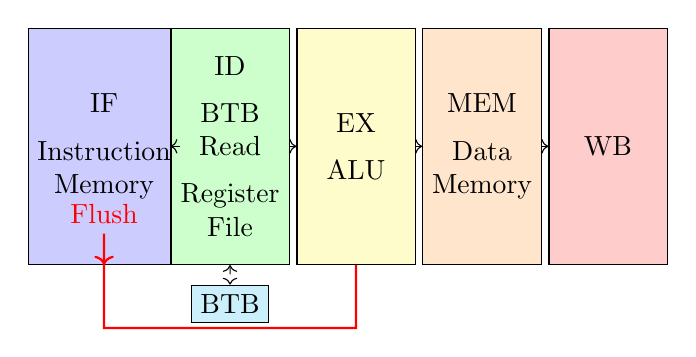
\begin{tikzpicture}[scale=0.8]
    % Pipeline stages
    \node[draw, rectangle, minimum width=1.5cm, minimum height=3cm, fill=blue!20, align=center] (if) at (0, 0) {IF\\[5pt]Instruction\\Memory};
    \node[draw, rectangle, minimum width=1.5cm, minimum height=3cm, fill=green!20, align=center] (id) at (2, 0) {ID\\[5pt]BTB\\Read\\[5pt]Register\\File};
    \node[draw, rectangle, minimum width=1.5cm, minimum height=3cm, fill=yellow!20, align=center] (ex) at (4, 0) {EX\\[5pt]ALU};
    \node[draw, rectangle, minimum width=1.5cm, minimum height=3cm, fill=orange!20, align=center] (mem) at (6, 0) {MEM\\[5pt]Data\\Memory};
    \node[draw, rectangle, minimum width=1.5cm, minimum height=3cm, fill=red!20, align=center] (wb) at (8, 0) {WB};
    
    % BTB
    \node[draw, rectangle, fill=cyan!20] (btb) at (2, -2.5) {BTB};
    
    % Connections
    \draw[->] (if) -- (id);
    \draw[->] (id) -- (ex);
    \draw[->] (ex) -- (mem);
    \draw[->] (mem) -- (wb);
    \draw[<->, dashed] (id) -- (btb);
    
    % Feedback path
    \draw[->, thick, red] (ex.south) -- ++(0, -1) -- ++(-4, 0) -- ++(0, 1.5) node[above] {Flush} -- (if.south);
\end{tikzpicture}
\end{center}

\textbf{Question:} How many clock cycles are wasted for correct prediction vs. misprediction?
\end{frame}

\begin{frame}{Pipeline Timing Analysis - Correct Predictions}
%\textbf{Branch Prediction: When We Get It Right}
\scriptsize
\vspace{0.3cm}

% Case 1: Correct Prediction - Not Taken (BEST CASE)
\begin{center}
\colorbox{green!10}{
\begin{minipage}{0.95\textwidth}
\textbf{Case 1: Correct Prediction - Not Taken} \hfill \textcolor{green!70!black}{\textbf{0 cycle penalty} $\checkmark$}
\vspace{0.1cm}

\begin{tabular}{l|c|c|c|c|c|c}
\textbf{Instruction} & \textbf{C1} & \textbf{C2} & \textbf{C3} & \textbf{C4} & \textbf{C5} & \textbf{C6} \\
\hline
beq & \cellcolor{normalexec!40}IF & \cellcolor{normalexec!40}ID & \cellcolor{normalexec!40}EX & \cellcolor{normalexec!40}MEM & \cellcolor{normalexec!40}WB & \\
next & & \cellcolor{normalexec!40}IF & \cellcolor{normalexec!40}ID & \cellcolor{normalexec!40}EX & \cellcolor{normalexec!40}MEM & \cellcolor{normalexec!40}WB \\
\end{tabular}

\vspace{0.05cm}
\footnotesize \textbf{Optimal:} No stall - same as original MIPS pipeline
\end{minipage}
}
\end{center}

\vspace{0.4cm}

% Case 2: Correct Prediction - Taken
\begin{center}
\colorbox{green!10}{
\begin{minipage}{0.95\textwidth}
\textbf{Case 2: Correct Prediction - Taken} \hfill \textcolor{orange!70!black}{\textbf{1 cycle penalty}}
\vspace{0.1cm}

\begin{tabular}{l|c|c|c|c|c|c|c}
\textbf{Instruction} & \textbf{C1} & \textbf{C2} & \textbf{C3} & \textbf{C4} & \textbf{C5} & \textbf{C6} & \textbf{C7} \\
\hline
beq & \cellcolor{normalexec!40}IF & \cellcolor{normalexec!40}ID & \cellcolor{normalexec!40}EX & \cellcolor{normalexec!40}MEM & \cellcolor{normalexec!40}WB & & \\
\textit{bubble} & & \cellcolor{stallcolor!40}--- & \cellcolor{emptycolor}--- & \cellcolor{emptycolor}--- & \cellcolor{emptycolor}--- & \cellcolor{emptycolor}--- & \\
target & & & \cellcolor{normalexec!40}IF & \cellcolor{normalexec!40}ID & \cellcolor{normalexec!40}EX & \cellcolor{normalexec!40}MEM & \cellcolor{normalexec!40}WB \\
\end{tabular}

\vspace{0.05cm}
\footnotesize \textbf{Good:} One bubble while waiting for target address from EX stage
\end{minipage}
}
\end{center}

\vspace{0.3cm}

\begin{tikzpicture}[remember picture, overlay]
    \node[anchor=south east, inner sep=8pt] at (current page.south east) {
        \begin{tabular}{ll}
        \footnotesize
        \cellcolor{normalexec!40} & Normal execution \\
        \cellcolor{stallcolor!40} & Stall/Bubble \\
        \cellcolor{emptycolor}--- & Empty stage \\
        \end{tabular}
    };
\end{tikzpicture}

\begin{center}
\large
\textcolor{green!70!black}{\textbf{When prediction is correct, penalty is minimal (0-1 cycles)}}
\end{center}

\end{frame}

% Second frame for mispredictions
\begin{frame}{Pipeline Timing Analysis - Mispredictions}
%\textbf{Branch Prediction: When We Get It Wrong}
\scriptsize
\vspace{0.3cm}

% Case 3: Misprediction - Predicted Not Taken, Actually Taken
\begin{center}
\colorbox{red!10}{
\begin{minipage}{0.95\textwidth}
\textbf{Case 3: Misprediction - Predicted Not Taken $\rightarrow$ Actually Taken} \hfill \textcolor{red!70!black}{\textbf{2 cycle penalty} \xmark}
\vspace{0.1cm}

\begin{tabular}{l|c|c|c|c|c|c|c|c}
\textbf{Instruction} & \textbf{C1} & \textbf{C2} & \textbf{C3} & \textbf{C4} & \textbf{C5} & \textbf{C6} & \textbf{C7} & \textbf{C8} \\
\hline
beq & \cellcolor{normalexec!40}IF & \cellcolor{normalexec!40}ID & \cellcolor{normalexec!40}EX & \cellcolor{normalexec!40}MEM & \cellcolor{normalexec!40}WB & & & \\
\textcolor{red}{next (wrong)} & & \cellcolor{normalexec!40}IF & \cellcolor{flushcolor!40}ID & \cellcolor{flushcolor!40}\textsf{X} & \cellcolor{emptycolor}--- & \cellcolor{emptycolor}--- & \cellcolor{emptycolor}--- & \\
\textcolor{red}{next+1 (wrong)} & & & \cellcolor{flushcolor!40}IF & \cellcolor{flushcolor!40}\textsf{X} & \cellcolor{emptycolor}--- & \cellcolor{emptycolor}--- & \cellcolor{emptycolor}--- & \\
target (correct) & & & & \cellcolor{normalexec!40}IF & \cellcolor{normalexec!40}ID & \cellcolor{normalexec!40}EX & \cellcolor{normalexec!40}MEM & \cellcolor{normalexec!40}WB \\
\end{tabular}

\vspace{0.05cm}
\footnotesize \textbf{Bad:} 2 instructions fetched incorrectly and must be flushed
\end{minipage}
}
\end{center}

\vspace{0.4cm}

% Case 4: Misprediction - Predicted Taken, Actually Not Taken
\begin{center}
\colorbox{red!10}{
\begin{minipage}{0.95\textwidth}
\textbf{Case 4: Misprediction - Predicted Taken $\rightarrow$ Actually Not Taken} \hfill \textcolor{red!70!black}{\textbf{2 cycle penalty} \xmark}
\vspace{0.1cm}

\begin{tabular}{l|c|c|c|c|c|c|c|c}
\textbf{Instruction} & \textbf{C1} & \textbf{C2} & \textbf{C3} & \textbf{C4} & \textbf{C5} & \textbf{C6} & \textbf{C7} & \textbf{C8} \\
\hline
beq & \cellcolor{normalexec!40}IF & \cellcolor{normalexec!40}ID & \cellcolor{normalexec!40}EX & \cellcolor{normalexec!40}MEM & \cellcolor{normalexec!40}WB & & & \\
\textit{bubble} & & \cellcolor{stallcolor!40}--- & \cellcolor{emptycolor}--- & \cellcolor{emptycolor}--- & \cellcolor{emptycolor}--- & \cellcolor{emptycolor}--- & & \\
\textcolor{red}{target (wrong)} & & & \cellcolor{normalexec!40}IF & \cellcolor{flushcolor!40}ID & \cellcolor{flushcolor!40}\textsf{X} & \cellcolor{emptycolor}--- & \cellcolor{emptycolor}--- & \\
next (correct) & & & & \cellcolor{normalexec!40}IF & \cellcolor{normalexec!40}ID & \cellcolor{normalexec!40}EX & \cellcolor{normalexec!40}MEM & \cellcolor{normalexec!40}WB \\
\end{tabular}

\vspace{0.05cm}
\footnotesize \textbf{Bad:} 1 stall cycle + 1 incorrectly fetched instruction flushed
\end{minipage}
}
\end{center}

\vspace{0.3cm}

\begin{tikzpicture}[remember picture, overlay]
    \node[anchor=south east, inner sep=8pt] at (current page.south east) {
        \begin{tabular}{ll}
        \footnotesize
        \cellcolor{normalexec!40} & Normal execution \\
        \cellcolor{stallcolor!40} & Stall/Bubble \\
        \cellcolor{flushcolor!40}\textsf{X} & Flushed \\
        \cellcolor{emptycolor}--- & Empty stage \\
        \end{tabular}
    };
\end{tikzpicture}

\begin{center}
\large
\textcolor{red!70!black}{\textbf{Mispredictions are costly - always 2+ cycle penalty}}
\end{center}

\end{frame}

\begin{frame}{Optimization: Avoiding Stalls on Correct Prediction}
\textbf{Problem:} One cycle stall even on correct "Taken" prediction

\textbf{Solution 1: Store Previous Instruction Address}
\begin{itemize}
    \item Store address of instruction BEFORE the branch in BTB
    \item When that instruction reaches ID, start BTB lookup
    \item Branch instruction will be in IF stage
    \item Achieves optimal timing (no stall on correct prediction)
\end{itemize}

\textbf{Challenge:} Programs may reach branch from different locations
\begin{center}
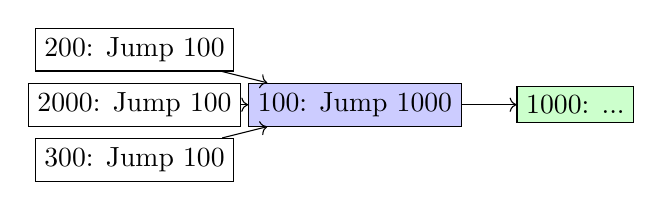
\begin{tikzpicture}[scale=0.7]
    \node[draw, rectangle] (j1) at (0, 2) {200: Jump 100};
    \node[draw, rectangle] (j2) at (0, 1) {2000: Jump 100};
    \node[draw, rectangle] (j3) at (0, 0) {300: Jump 100};
    \node[draw, rectangle, fill=blue!20] (target) at (4, 1) {100: Jump 1000};
    \node[draw, rectangle, fill=green!20] (dest) at (8, 1) {1000: ...};
    
    \draw[->] (j1) -- (target);
    \draw[->] (j2) -- (target);
    \draw[->] (j3) -- (target);
    \draw[->] (target) -- (dest);
\end{tikzpicture}
\end{center}

\textbf{Solution 2:} Store target instruction itself in BTB (saves IF stage)

\textbf{Solution 3:} Move BTB lookup to IF stage with specialized hardware
\end{frame}

\begin{frame}[fragile]{Complex Example: Exam Question}
\begin{columns}
\column{0.5\textwidth}
\begin{lstlisting}[language={[x86masm]Assembler}]
place2: 
    ADDI R4,R4,#2
    ADDI R4,R4,#2
    LD R10,R4(128)
    ADDI R9,R9,#0
    BEQ R10,R1,place1
    ADDI R7,R7,#1
place1: 
    BNEQ R10,R1,place2
    ADDI R8,R8,#1
\end{lstlisting}

\column{0.5\textwidth}
\textbf{Given:}
\begin{itemize}
    \item MIPS-like processor
    \item Branch decision in EX stage
    \item BTB lookup in IF stage
    \item BTB contains both branch instructions
    \item Predictions are correct
    \item BNEQ is taken
\end{itemize}
\end{columns}

\vspace{0.3cm}
\textbf{Question:} How many cycles for first iteration starting from place2?

\textbf{Answer:} 7 cycles (7 instructions in the iteration)
\end{frame}

\begin{frame}{Complex Example: Analysis}
\textbf{\ding{193}} If the entire code takes 33 cycles, how many times was LD executed?

\textbf{Analysis:}
\begin{itemize}
    \item Last iteration: BNEQ not taken $\Rightarrow$ BEQ taken
    \item Each iteration has 7 instructions
    \item Each misprediction costs 2 cycles
    \item Pipeline fill needs 4 cycles
\end{itemize}

\textbf{Formula:}
$$7 \times \text{\#iterations} + 2 \times \text{\#mispredictions} + 4 = 33$$

Since each iteration has 2 branch instructions:
$$2 \times \text{\#iterations} \geq \text{\#mispredictions}$$

\textbf{Solution:} \#iterations = 3, \#mispredictions = 4
$\Rightarrow$ LD executed \textbf{3 times}
\end{frame}

\begin{frame}{State Machine Configuration}
\textbf{\ding{194}} Design a state machine that produces 4 mispredictions in 6 branch executions (3 iterations)

\pause
\begin{center}
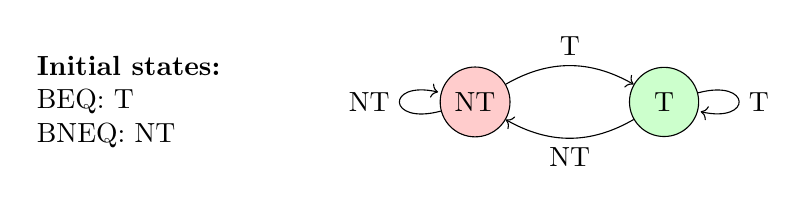
\begin{tikzpicture}[scale=0.8, node distance=2.5cm]
    % State machine for demonstration
    \node[state, fill=red!20] (nt) at (0, 0) {NT};
    \node[state, fill=green!20] (t) at (3, 0) {T};
    
    \path[->] 
    (nt) edge[bend left, above] node{T} (t)
    (t) edge[bend left, below] node{NT} (nt)
    (nt) edge[loop left] node{NT} (nt)
    (t) edge[loop right] node{T} (t);
    
    % Initial states on the left
    \node[align=left] at (-5.5, 0) {\textbf{Initial states:}\\BEQ: T\\BNEQ: NT};
\end{tikzpicture}
\end{center}
\begin{columns}
\column{0.2\textwidth}
\textbf{Execution Trace:}
\column{0.8\textwidth}
\begin{table}
\centering
\scriptsize
\begin{tabular}{|c|c|c|c|}
\hline
\textbf{Iteration} & \textbf{Instruction} & \textbf{Prediction} & \textbf{Actual} \\
\hline
1 & BEQ & T & NT \\
1 & BNEQ & NT & T \\
2 & BEQ & NT & NT \\
2 & BNEQ & T & T \\
3 & BEQ & NT & T \\
3 & BNEQ & T & NT \\
\hline
\end{tabular}
\end{table}
\end{columns}

Result: 4 mispredictions, 2 correct predictions
\end{frame}

\begin{frame}{Summary}
\textbf{Key Concepts:}
\begin{itemize}
    \item \textbf{BTB (Branch Target Buffer)} stores:
    \begin{itemize}
        \item Branch instruction addresses
        \item Target addresses
        \item Prediction state (1-bit or 2-bit)
    \end{itemize}
    \item \textbf{2-bit predictors} provide better accuracy by requiring two consecutive mispredictions to change stable state
    \item \textbf{Pipeline integration} affects performance:
    \begin{itemize}
        \item BTB lookup stage determines stall cycles
        \item Branch resolution stage determines misprediction penalty
    \end{itemize}
    \item \textbf{Optimizations} can eliminate stalls on correct predictions
\end{itemize}

\textbf{Performance Impact:}
\begin{itemize}
    \item Correct prediction (Taken): 0-1 cycle penalty
    \item Correct prediction (Not Taken): 0 cycle penalty
    \item Misprediction: 2+ cycle penalty (depends on pipeline depth)
\end{itemize}
\end{frame}

\end{document}